In order to address both I/O and in situ analysis/visualization issues,
we propose to gather the I/O operations into a set of dedicated cores in each
multicore node. These cores (typically one per node)
are dedicated to data management tasks (i.e., they do not run the simulation code) in order
to overlap writes and analysis tasks with computation and avoid contention for accesses
to the file system. The cores running the simulation
and the dedicated cores communicate data through shared memory.
We call this approach Damaris. Its design, implementation and API are described below.

\subsection{Design Principles}

The Damaris approach is based on four main design principles.

\subsubsection{Dedicated Cores}

The Damaris approach is based on a set of processes running on dedicated cores in every multicore node.
Each dedicated core performs in situ processing and I/O in response to user-defined events sent by the simulation.
We call a process running the simulation a \emph{client}, and a process running on a dedicated core a \emph{server}.
One important aspect of Damaris is that dedicated cores do not run the simulation.
With the current trend in hardware solutions, the number of cores per node increases.
Thus dedicating one or a few cores has a diminishing impact on the performance of the simulation. 
Hence, our approach primarily targets SMP nodes featuring a large number of cores per node: 12 to 24 in our experiments.

\subsubsection{Data Transfers through Shared Memory}

Damaris handles large data transfers from clients to servers through shared memory.
This makes a write as fast as a \texttt{memcpy} and also enables direct allocation of
variables within the shared memory. This option is especially useful to reduce the
memory requirements of in situ visualization tasks, which can directly access the memory
of the simulation without requiring a copy (see our previous work~\cite{dorier2013damarisviz}).

\subsubsection{High-Level Data Abstraction}

Clients write enriched datasets in a way similar to scientific I/O libraries such as HDF5~\cite{folk1999hdf5} or NetCDF~\cite{netcdf}.
That is, the data output by the simulation is organized into a hierarchy of groups and variables,
with additional metadata such as the description of variables, their type, unit, and layout in memory.
The dedicated cores thus have enough knowledge of incoming datasets to write them in existing high-level 
formats. This design principle differs from other approaches that capture I/O operations at a lower 
level~\cite{li2010functional,ma2006highlevel}. These approaches indeed lose the semantics of the data being written.
While our design choice forces us to modify the simulation so that it writes its data using Damaris' API,
is allows to implement semantic-aware data processing functionalities in dedicated cores. In particular, keeping
this level of semantics is mandatory in order for dedicated cores to be able to write data in a standard, high-level
format such as HDF5 or NetCDF, or to feed an in situ visualization pipeline.

\subsubsection{Extensibility through Plugins}

Servers can perform data transformations prior to writing them, as well as analysis and visualization.
One major design principle in the Damaris approach is the possibility for users to provide these 
transformations through a plugin system, thus adapting Damaris to the particular requirements of 
their application. Implementing such a plugin system at a lower level would
not be possible, as it would not have access to the high-level information about
the data (e.g., dimensions of arrays, data types, physical meaning of the variable 
within the simulation, etc.).

\subsection{Architecture}

\begin{figure}
	\begin{center}
	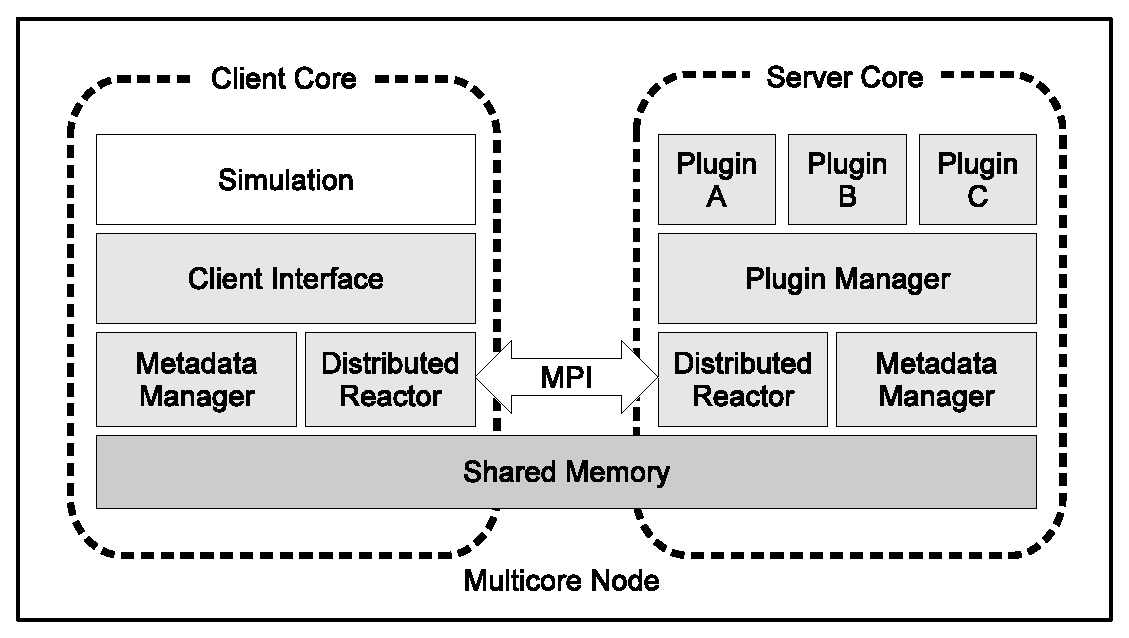
\includegraphics[width=\textwidth]{figures/damaris-schema.eps}
	\caption[Software architecture of the implementation of Damaris]{Software architecture of the implementation of Damaris.}\label{fig:damaris:design}
	\end{center}
\end{figure}

Figure~\ref{fig:damaris:design} presents the software architecture underlying the Damaris approach.
While Damaris can dedicate several cores in large multicore nodes, only one client
and one server are represented here.

Damaris has been designed in a highly modular way and features
a number of decoupled, reusable software components.
The \emph{Shared Memory} component handles the shared buffer and ensures the safety of
concurrent allocations/deallocations. The \emph{Distributed Reactor} handles communications between 
clients and servers, and across servers. The \emph{Metadata Manager} stores high-level information 
related to the data being transferred (type, size, layout, etc.).
Finally the \emph{Plugin Manager} on the server side loads and runs user-provided plugins.

This modular architecture greatly simplified the
adaptation to several HPC platforms and simulations, as well as the development of
extensions to support various scenarios such as storage, in situ visualization, data compression 
or I/O scheduling. The following sections describe each component in more detail.

\subsubsection{Shared Memory}

Data communications between the clients and the servers are
performed through the Shared Memory component. A large
memory buffer is created on each node by the dedicated cores at start time, with a size set by the user 
(typically several MB to several GB). 
Thus the user has full control over the resources allocated to Damaris.
When a client submits new data, it reserves a segment of this shared-memory buffer. 
It then copies its data using the returned pointer so that the local memory can be reused.

\subsubsection{Distributed Reactor}

The Distributed Reactor is the most complex component of Damaris.
It builds on the \emph{Reactor} design pattern~\cite{coplien95reactor} to provide the means 
by which different cores (clients and servers) communicate. 
Reactor is a behavioral pattern that handles requests concurrently sent to an application by one or more clients.
The Reactor asynchronously listens to a set of \emph{channels} connecting it to its clients.
The clients send small events that are associated with event handlers (i.e., functions) in the Reactor.
A synchronous event demultiplexer is in charge of queuing the events received by the Reactor and calling 
the appropriate event handlers.

Contrary to a normal Reactor design pattern (as used in \emph{Boost.ASIO}\footnote{See \url{http://www.boost.org/}} for example), 
our Distributed Reactor also provides elaborate collective operations.
%
\begin{description}
	\item[Asynchronous atomic multicast:] A process can broadcast an event to a group
	of processes at once. This operation is asynchronous, that is, the sender does not wait
	for the event to be processed by all receivers to resume its activity. A receiver
	only processes the event when all other receivers are ready to process it as well.
	It is also atomic, that is, if two distinct processes broadcast a different event, the
	Distributed Reactor ensures that all receivers will handle the two events in the same order.
	
	\item[Asynchronous atomic labeled barrier:] We call a ``labeled'' barrier across a set of
	processes a synchronization barrier associated with an event (its label). After all processes reach the barrier, 
	they all invoke the event handler associated with the event. 
	This ensures that all processes agree to execute the same code at 
	the same \emph{logical} time. This primitive is asynchronous: it borrows its semantics 
	from MPI~3's \texttt{MPI\_Ibarrier} non-blocking barrier.
	It is atomic according to the same definition as the asynchronous atomic multicast.
\end{description}
%
These two distributed algorithms are very important in the design of in situ processing tasks
that include communications between servers. In particular, they ensure that plugins will
be triggered in the same order in all servers, allowing collective communications to safely
take place within these plugins.

\subsubsection{Metadata Manager}

The Metadata Manager component keeps information related to the data
being written, including \emph{variables}, \emph{layouts} (describing the type and shape of
blocks of data), \emph{parameters}, etc. It is initialized using an XML configuration file.

This design principle is inspired by ADIOS~\cite{lofstead2008flexible} 
and other tools such as EPSN~\cite{esnard2006steering}.
In traditional data formats such as HDF5, several functions have to be called by the
simulation to provide metadata information prior to actually writing data.
The use of an XML file in Damaris presents several advantages.
First, the description of data provided by the configuration file can be changed without 
changing the simulation itself, and the amount of code required to use Damaris in a simulation
is reduced compared to existing data formats.
Second, it prevents clients from transferring metadata to dedicated cores through shared memory. 
Clients communicate only data along with the minimum information
required by dedicated cores to retrieve the full description in their own Metadata Manager.

Contrary to the XDMF format~\cite{xdmf}, which leverages XML to store scientific datasets
along with metadata (or points to data in external HDF5 files), our XML file only provides metadata related to
data produced by the simulation. It is not intended to be an output format, or become part of one.

\subsubsection{Plugin Manager}

The Plugin Manager is the component that loads and stores plugins.
Plugins are pieces of C++ or Python codes provided by the user. The Plugin Manager is capable of
loading functions from dynamic libraries or scripts as well as from the simulation's code itself. 
It is initialized from the XML configuration file. Again, the use of a common
configuration file between clients and servers allows different processes
to refer to the same plugin through an identifier rather than its full name and attributes.

A server can call a plugin when it receives its corresponding event, or
wait for all clients in a node or in the entire simulation to have sent the event. 
In these later cases, the collective algorithms provided by the Distributed Reactor ensure that
all servers call the plugins in the same order.

\subsection{Implementation}

The Damaris approach is intended to be the basis for a generic, platform-independent,
application-independent, easy-to-use tool. This section describes its main API and
provides some technical details of its implementation.

\subsubsection{Client API}

%%%%%%%%%%%%%%%%%%%%%%%%%%%%%%%%%%%%%%%%
Our implementation provides client-side interfaces for C, C++ and Fortran applications written with MPI.
This API can be summarized by the following functions.
%
\begin{itemize}
	\item \texttt{damaris\_initialize("config.xml")}
	initializes the resources used by Damaris using the configuration file given as parameter. 
	All cores (clients and servers) call this function at the beginning of the simulation.
	
	\item \texttt{damaris\_start()} is called by all cores to start servers on dedicated cores. 
	The servers block within this function, while the clients return and proceed with the simulation.
	
	\item \texttt{damaris\_get\_client\_comm()} provides an MPI communicator gathering
	only clients. Indeed the MPI\_COMM\_WORLD communicator contains both clients and servers
	 and cannot be used by the simulation anymore for its collective communications.
	
	\item \texttt{damaris\_write("var\_name",data)} is called by clients. It copies the data in shared 
	memory along with minimal information and notifies the server on the same node. 
	All additional information such as the size of the data and its layout 
	can be found by the servers in the configuration file.
	
	\item \texttt{damaris\_alloc("variable")} is similar to \emph{malloc} (or 
	\emph{allocate} in Fortran, \emph{new} in C++). It is called by clients to allocate a portion of 
	shared memory to hold the variable for a given iteration and returns a 
	pointer. Only the simulation is aware of this allocation, dedicated cores
	cannot access the data. The returned buffer is expected to be used as output buffer for the
	next iteration.
	
	\item \texttt{damaris\_commit("variable")} is called by clients when the simulation has
	finished writing to the current buffer associated with the variable. It 
	sends the location of the data to the dedicated cores. Both the simulation 
	and dedicated cores can read the data. At this point, clients will use the buffer as input
	for the next iteration while dedicated cores will use it as input for visualization tasks.
	
	\item \texttt{damaris\_clear("variable")} is called by clients to notify the dedicated cores that the 
	committed data for this variable will no longer be used by the simulation. 
	It can safely be processed, stored or removed from shared memory. The clients will issue another
	\texttt{damaris\_alloc} to get a new portion of shared memory to use as output buffer.
	
	\item \texttt{damaris\_signal("event\_name")} is called by clients to send a custom event
	to the server in order to trigger a plugin predefined in the configuration file.
	
	\item \texttt{damaris\_end\_iteration()} notifies the servers that the
	simulation has reached the end of an iteration and will start the next one. This allows
	dedicated cores to know that the data written in shared memory is consistent and nothing
	more should be expected for this iteration.
	
	\item \texttt{damaris\_stop()} stops the servers on dedicated cores, making them leave
	the \texttt{damaris\_start} function.
	
	\item \texttt{damaris\_finalize()} frees the resources used by Damaris. It is called by
	all processes after servers have been stopped on dedicated cores (using \texttt{damaris\_stop})
	before terminating the simulation.
\end{itemize}

\subsubsection{Technical Implementation Details}

Damaris leverages the \textit{Boost.Interprocess} 
library\footnote{See \url{http://www.boost.org/}} to implement several versions of the Shared Memory component,
suitable for different platforms.

Our implementation of the Distributed Reactor relies on MPI~2 communication
primitives and, in particular, non-blocking \emph{send} and \emph{receive} operations. Events are simply
implemented as 0-byte messages with the MPI \emph{tag} carrying the type of the event. Since the MPI~3 standard
provides new non-blocking collective functions such as \texttt{MPI\_Ireduce} or \texttt{MPI\_Ibarrier},
our Distributed Reactor could be easily re-implemented with these MPI~3 functions without any impact on the
rest of Damaris' implementation.

Finally we used Model-Driven Engineering (MDE) techniques to implement the Metadata Manager.
Most of the source code of the Metadata Manager is indeed automatically generated from an XSD metamodel. 
This metamodel describes the concepts of \emph{variables}, \emph{layouts}, etc. 
as well as their relations to one another and how they are described in an XML format.
The XSD file is used to synthesize C++ classes that correspond to the metamodel.

\subsection{Managing Data with Damaris}

Damaris is not a data format. It only provides a framework to
dedicate cores for custom data processing and I/O tasks, to transfer data through shared memory and to call plugins.
Thanks to its plugin system, Damaris can be adapted to many scenarios of in situ data processing.
In this paper, we specifically use it to periodically write data and to perform in situ visualization.

\subsubsection{Writing Data}

We implemented a plugin that gathers data from client cores and writes
them into HDF5 files. Each server running on a dedicated core produces a single file per iteration.
Compared with the file-per-process approach, this way of writing produces fewer, bigger files, thus
mitigating the bottleneck in metadata servers when files are created. Writing from a reduced
number of writers also has the advantage of limiting network access contention across the cores of
the same node. Finally, issuing bigger writes to the file system usually allows for better performance.
Compared with the collective I/O approach, our writer plugin does not require synchronization between
processes.

\subsubsection{Visualizing and Analyzing}

The high-level data description provided by Damaris enables a connection with  
existing visualization and analysis packages, including VisIt~\cite{visit} or ParaView~\cite{paraview}, in order to build 
a full in situ visualization framework.
Both VisIt and ParaView perform in situ visualization from in-memory data. 
Given that each of these software has strengths, a major advantage of
our approach is the ability to switch between them with no code modification in the simulation.
%

%
%\begin{Listing}[h]
%	\lstinputlisting[language=XML]{listings/damaris_mesh.xml}
%	\caption[Description of a mesh in the Damaris/Viz %configuration]{Description of a mesh in the Damaris/Viz configuration.}
%	\label{lst:damarismeshxml}
%\end{Listing}
%
%\begin{Listing}
%	\lstinputlisting[language=C]{listings/damaris_access.c}
%	\caption[Allocation for data accessed by Damaris]{Allocation for data accessed by Damaris. 
%	The size is given in the Damaris configuration file.}\label{lst:damarisaccess}
%\end{Listing}
%
We leveraged the XSD-based metadata management in Damaris to provide the
necessary information to bridge simulations to existing visualization 
software. By investigating the in situ interfaces of different visualization 
packages including ParaView, VisIt, ezViz~\cite{ezviz} and VTK~\cite{schroeder2000visualizing}, 
we devised a generic description of visualizable structures such as meshes, points or curves.
Additionally, the Distributed Reactor enables synchronization between dedicated cores,
which is necessary to run the parallel rendering algorithms implemented by the aforementioned visualization software.

\subsection{Code Sample using Damaris}\label{sec:damaris_viz:DamarisInSitu}

\begin{SCfigure}
	\centering
	\caption{Example of a $4\times4\times4$ rectilinear grid described by three arrays
	of coordinates. In this example there is a 
	scalar value (such as \emph{temperature} or \emph{wind velocity}) at each node. The mesh itself
	is described through three coordinate arrays:
	\texttt{mesh\_x = \{0.0,1.0,2.0,3.0\}; mesh\_y = \{0.0,1.0,2.0,3.0\}; mesh\_z = \{0.0,1.2,1.8,3.0\}}.
	}
	\label{fig:mesh}
	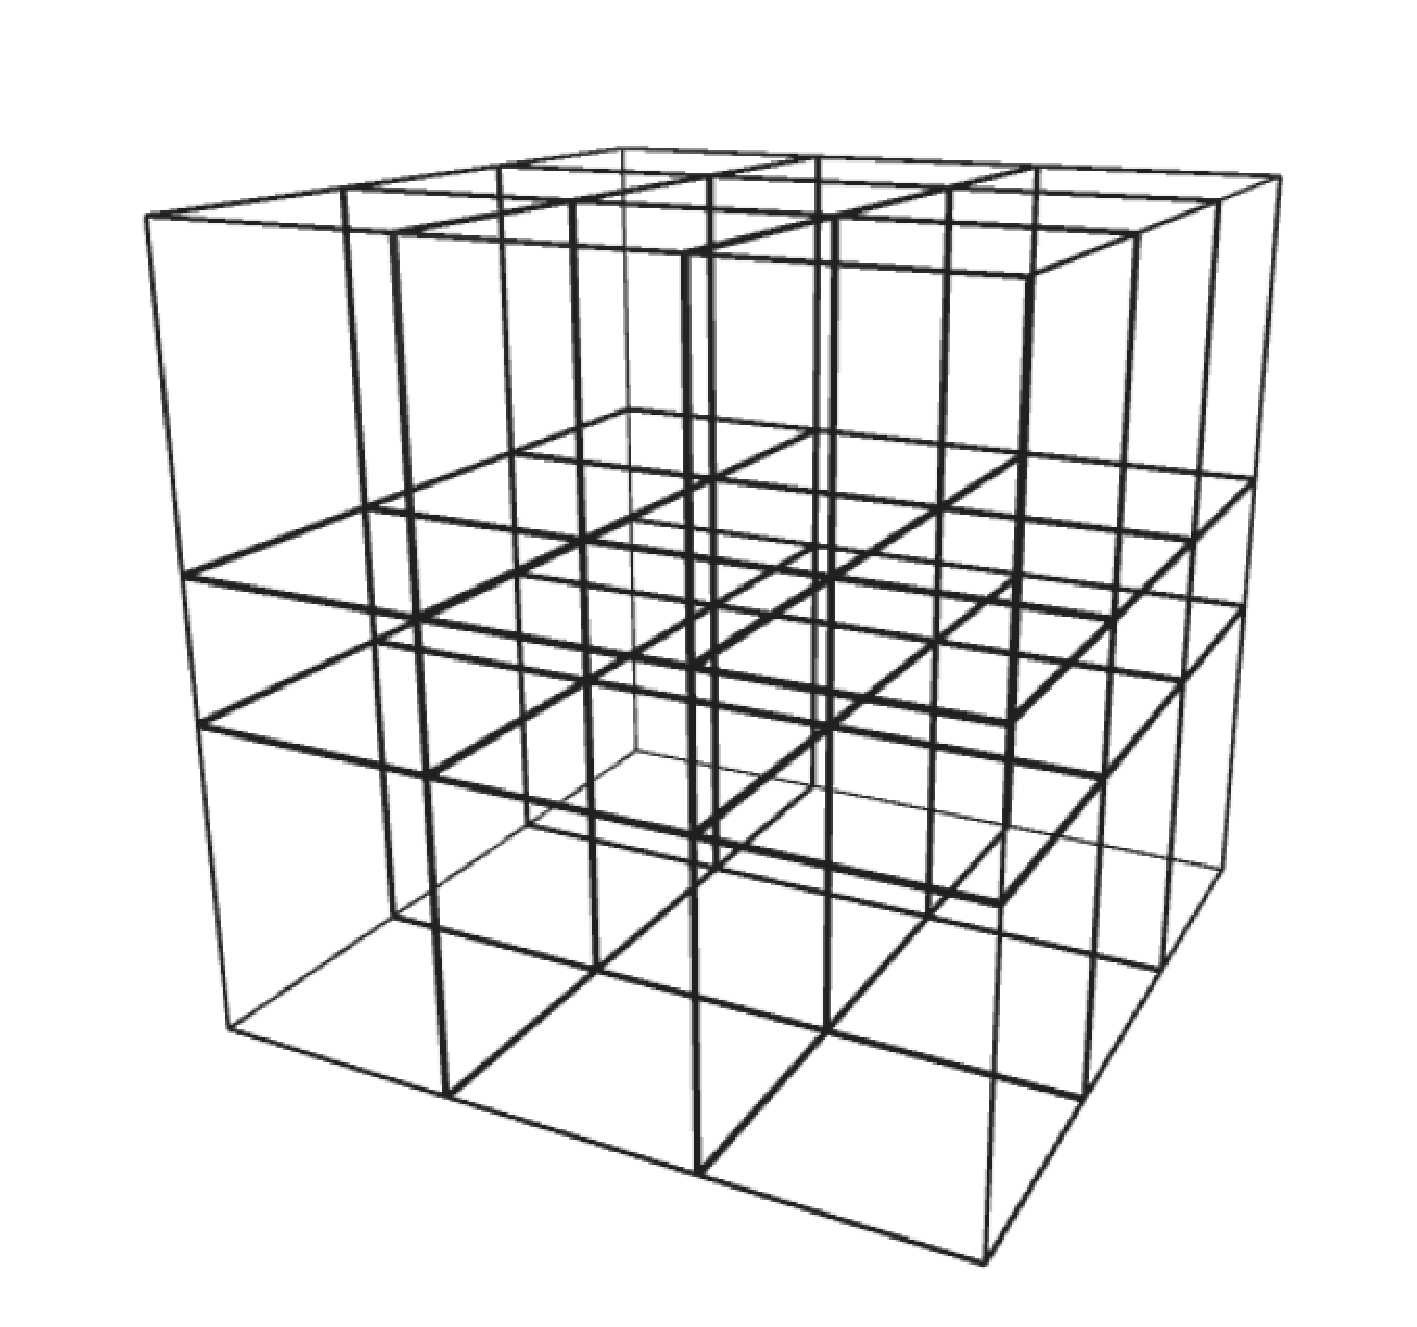
\includegraphics[width=7cm]{figures/mesh.eps}
\end{SCfigure}

\begin{Listing}[h]
	\lstinputlisting[language=fortran]{listings/damaris_example.f90}
	\caption[Example of Fortran simulation using Damaris]{Example of Fortran simulation using Damaris.}
	\label{lst:damarisexample}
\end{Listing}

\begin{Listing}[h]
	\lstinputlisting[language=XML]{listings/damaris_example.xml}
	\caption[Configuration file associated with the Fortran example]{Configuration file associated with the Fortran example.}
	\label{lst:damarisexamplexml}
\end{Listing}

Listing~\ref{lst:damarisexample} is an example of a Fortran program 
that makes use of Damaris. It writes three 1D arrays representing the coordinates of a rectilinear mesh.
At every iteration it then writes
a 3D array representing temperature values on the points of the mesh and sends an event to the dedicated core.
The associated configuration file, shown in Listing~\ref{lst:damarisexamplexml},
describes the data that is expected to be received by the servers, and the
action to perform upon reception of the event. More specifically, lines~14, 15, 16 and 18 of this XML file 
define \emph{layouts}, which describe the type and dimensions of a piece of data. Lines~26 to 33 define a group,
and within this group a set of variables that use these layouts. The temperature variable is defined in line 35.
Finally line~38 associates an event with a function (or \emph{action}) to be
called when the event is received. It also locates the function within a dynamically-loaded library.

The configuration file also contains information for visualization software.
Lines~20 to 24 in the XML file correspond to mesh structure drawn in 
Figure~\ref{fig:mesh}, and built from the three coordinate variables. 
The temperature variable is mapped onto this mesh using its \emph{mesh} attribute.
